\section{Body Coordinate System}\label{sec:body}
This frame has also the origin in the center of gravity of the UA, however, unlike the vehicle-carried NED, the axis rotate with the craft:
\begin{itemize}
\item{The origin (\textbf{$O_{b}$}) is located at the center of gravity of the UA.}
\item{The X-axis (\textbf{$X_{b}$}) points in the forward direction.}
\item{The Y-axis (\textbf{$Y_{b}$}) points towards starboard, the right side of the UA.}
\item{The Z-axis (\textbf{$Z_{b}$}) points downward, set by the right-hand rule.}
\end{itemize}
\begin{figure}[H]
   \centering
    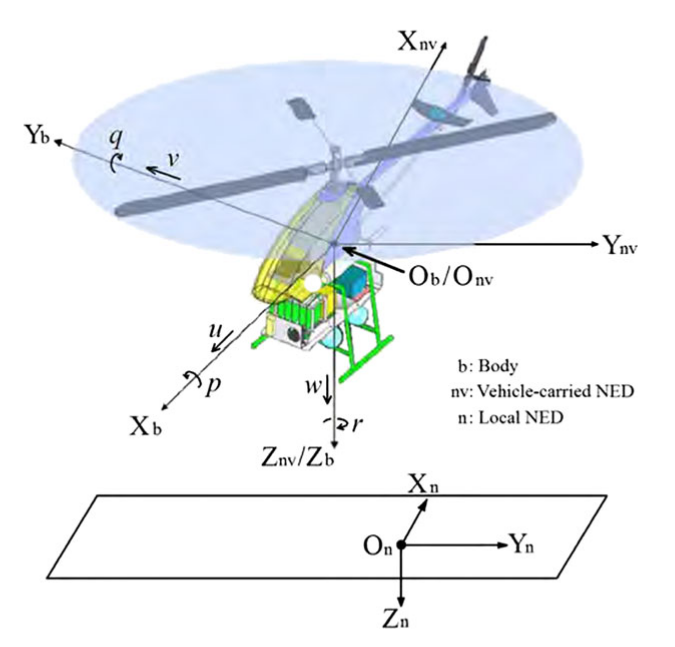
\includegraphics[width=.70\textwidth]{figures/NEDtemp1.png} 
    \caption{Body, vehicle-carried and local NED Frames.}  
    \label{fig:NED1}
\end{figure}

\section{Transformations}\label{sec:body}

\subsection*{From NED to Body}
\paragraph{} The orientation of a Cartesian coordinate system with respect to another can be described in three successive Euler rotations, usually performed about each of the three cartesian axes consequently. During this work we will mainly focus on the transformation between the vehicle-carried NED and the body frame. In order to do this we will follow a specific rotation sequence, moving the reference frame to the referred frame by a Z-Y-X (also called 3-2-1) sequence. These three Euler angles are also known respectively as \textbf{yaw}($\psi$), \textbf{pitch}($\xi$) and \textbf{roll}($\gamma$).

\paragraph{} This way, the transformation from the vehicle-carried NED frame to the Body frame is given by:
\begin{align}
\textbf{P}_{b} = \textbf{R}_{b/nv}\textbf{P}_{nv}
\end{align}
where \textbf{R}$_{b/nv}$ is the \textbf{Rotation matrix}:
\begin{align*}
\textbf{R}_{b/nv} =
\begin{bmatrix}
c(\xi)c(\psi) & c(\xi)s(\psi) & -s(\xi)\\
s(\gamma)s(\xi)c(\psi) - c(\gamma)s(\psi) & s(\gamma)s(\xi)s(\psi) + c(\gamma)c(\psi) & s(\gamma)c(\xi)\\
c\gamma)s(\xi)c(\psi) + s(\gamma)s(\psi) & c(\gamma)s(\xi)s(\psi) - s(\gamma)c(\psi) & c(\gamma)c(\xi)
\end{bmatrix}
\end{align*}

\paragraph{} However, even though the local NED coordinates is what is necessary to transform to the Body frame, the only available resource  is the GPS position measurements of each of our devices (Ground station and UA). Therefore a transformation from Geodetic Coordinate Frame to local NED frame is in due. The ECEF Coordinate Frame will be used as an intermediate step during this process.

\subsection*{From Geodetic to ECEF}
Being \textbf{P}$_{g}$ the position of a point in the geodetic system such that is defined by its latitude, longitude and height:
\begin{align}
\textbf{P}_{g} = 
\begin{bmatrix}
\lambda \\
\varphi\\
h
\end{bmatrix}
\end{align}
By using the parameters set by the \textbf{WGS84} standard in Section \ref{sec:geodetic} the transformed point, \textbf{P}$_{e}$ will be given by
\begin{align}
\textbf{P}_{e} = 
\begin{bmatrix}
\lambda \\
\varphi\\
h
\end{bmatrix}
=
\begin{bmatrix}
(N_{E}+h)c(\varphi)c(\lambda) \\
(N_{E}+h)c(\varphi)s(\lambda) \\
(N_{E}(1-\textbf{e}^2)+h)s(\varphi)
\end{bmatrix}
\end{align}

\subsection*{From ECEF to NED}
Analogously to the former transformation, we have
\begin{align}
\textbf{P}_{n} = \textbf{R}_{n/e}\left(\textbf{P}_{e} - \textbf{P}_{e,ref}\right)
\end{align}
where \textbf{P}$_{e,ref}$ is the position of the origin of the local NED frame in ECEF frame and \textbf{R}$_{n/e}$ is the \textbf{Rotation matrix} given by: 
\begin{align*}
\textbf{R}_{n/e} =
\begin{bmatrix}
-s(\varphi_{ref})c(\lambda_{ref}) & -s(\varphi_{ref})s(\lambda_{ref}) & c(\varphi_{ref})\\
-s(\lambda_{ref}) & c(\lambda_{ref}) & 0\\
-c(\varphi_{ref})c(\lambda_{ref}) & -c(\varphi_{ref})s(\lambda_{ref}) & -s(\varphi_{ref})\\
\end{bmatrix}
\end{align*}
where $\varphi_{ref}$ and $\lambda_{ref}$ are the latitude and longitude of the reference point in Geodetic frame.